%%\vspace{-5pt}
%\section{Introduction}
%%\vspace{-5pt}
%\label{interpretability_crr_sec:introduction}

\label{chapter:crr}
%The widespread adoption of prediction systems in various safety-critical domains such as medical diagnosis, law, education, and many others has led to the increased importance of presenting the decision functions in interpretable representations~\cite{K2001,MVBB2005,SAD2015,S2014,TV2013}.  To enable  safe, robust, and trustworthy integration of such systems, the end users require them to support interpretability, privacy, and fairness in decision-making~\cite{DF2018,VML2012,WRLKM2015,ZUR2017}. In this context,  rule-based representations are considered interpretable in presenting the decision functions to users~\cite{LKCL2019,WR2015,WRDLKM2017}. A recent body of work has studied sparsity-inducing objectives for classification rules in CNF or DNF and demonstrated that they often achieve high interpretability\textemdash defined in terms of rule-sparsity\textemdash with a minimal sacrifice in classification accuracy ~\cite{GM2019,LKCL2019,MM18}. 


In this chapter, we focus on improving the expressiveness of interpretable rule-based classifiers. Continuing on chapter~\ref{chapter:imli},
although CNF/DNF rules are considered interpretable, they are less expressive compared to Boolean cardinality constraints in propositional logic. A Boolean cardinality constraint allows one to express numerical bounds on Boolean variables~\cite{sinz2005towards}. In this chapter, we introduce a novel formulation of interpretable classification rules, namely \emph{relaxed-CNF}, which achieve benefits of  both worlds: it is interpretable similar to CNF/DNF  but more expressible by allowing cardinality constraints in the representation.


We find the motivation of relaxed-CNF rules from checklists. A checklist is a list of conditions that one needs to check, e.g., a list of items to take on a travel trip.  Checklists have several applications in interpretable decision making~\cite{M1976,gage2001validation}, particularly in the medical domain. For example, the  CHADS2 score in medicine is a clinical prediction rule for estimating the risk of stroke~\cite{gage2001validation}. Another example of checklists is a psychometric test, known as Myers–Briggs Type Indicator (MBTI)~\cite{M1976}, which indicates differing psychological preferences in how people perceive the world around them and make decisions.  An influential study on the importance of {checklists}~\cite{G2010} finds that highly complex and specialized problems can be handled smoothly by the development and consistent usage of checklists, which we formally call as relaxed-CNF rules. 


We now provide an introduction to relaxed-CNF rules. In interpretable rule-based classification, the simplest logical rules are single level-rules: ORs or ANDs of Boolean \textit{literals}, where each literal denotes either a Boolean input feature or its negation. A \emph{clause} is a collection of $ N $ literals connected by  OR/AND. To satisfy a clause, an OR operator requires $ 1 $ out of $ N $ literals to be assigned to  $ 1 $ in the clause, while an AND operator requires all $N$ out of $N$ literals to be assigned to  $ 1 $. A CNF   formula  is a conjunction (AND) of {clauses} where each clause is a disjunction (OR) of {literals}, and  a DNF  formula is a disjunction of clauses where each clause is a conjunction of literals. Therefore, CNF  and DNF  formulas can be viewed as two-level rules with several applications in interpretable decision-making. For example, a decision set is a DNF rule referring to a set of ``if-else'' conditions~\cite{ignatiev2018sat,lakkaraju2016interpretable}.  In this chapter, we consider a richer set of logical formulas that capture the structure of checklists. To this end, we consider \emph{hard}-OR clauses, where at least $ M > 1$ out of $ N $ literals are assigned to $ 1 $, and we similarly define {\emph{soft}-AND} clauses which allow some of the literals (at most $ N-M $) to be $ 0 $. To be precise,  the definitions of hard-OR and soft-AND overlap. Consequently, we use hard-OR when $M \le N/2$ and soft-AND otherwise. To extend the standard definition of CNF (which is ANDs of ORs),  we define \emph{relaxed}-CNF to denote soft-ANDs of hard-ORs. Similarly, \emph{relaxed}-DNF is hard-ORs of soft-ANDs. Since   hard-OR and soft-AND are differentiated based on the value of $ M $ and $ N $, relaxed-CNF and relaxed-DNF have the same structural representation. In early work, Craven and Shavlik~\cite{craven1996extracting} considered single level $ M $-of-$ N $ rules to explain black-box neural-network classifiers. Recently, Emad et al.~\cite{EVM2015} have developed a semi-quantitative group testing approach for learning sparse single level $M$-of-$N$ rules, which are quite restrictive in their ability to fit the data. In contrast, in this chapter, we study a much richer family of two-level relaxed-CNF rules. 





\begin{figure*}
	\begin{center}
		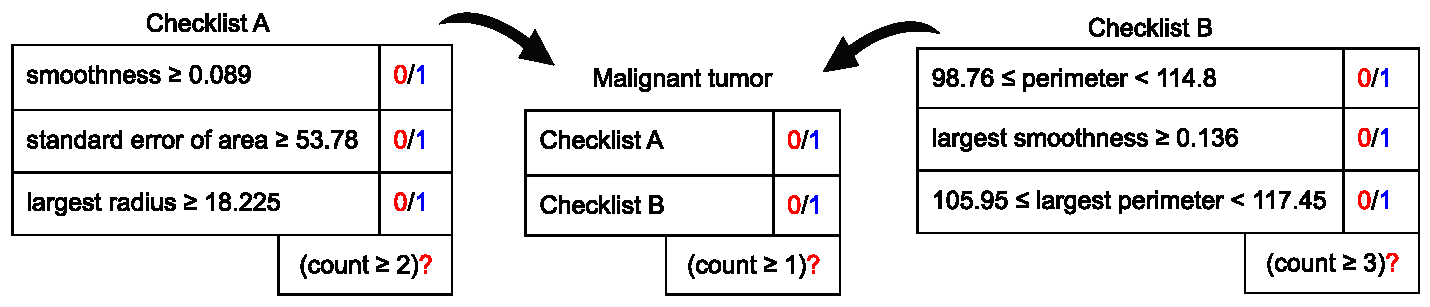
\includegraphics[scale=.62]{figures/interpretability/relaxed-cnf/checklist.pdf}
	\end{center}
	\caption[Illustration of a relaxed-CNF classification rule]{An illustrative example of a  relaxed CNF classification rule, which describes the decision function in the form of a  two-level checklist. This classifier is learned on the WDBC (Wisconsin diagnostic breast cancer) dataset and it predicts whether a tumor cell is malignant or not based on the characteristics of the  tumor cell. The first column in each checklist contains Boolean literals. An entry in the second column is  $ 1 $ if the corresponding literal is true by an observed tumor cell, and $ 0 $ otherwise. In the first level, checklist A (resp.\ B) is true if the count of true  literals is at least $ 2 $ (resp.\ $ 3 $). In the second level, a tumor cell is predicted as malignant if the count of true checklists is at least $ 1 $. }
	\label{interpretability_crr_exmpl:wdbc}
\end{figure*}




 {Relaxed-CNF rules are  more flexible than pure CNF rules, and they can accurately fit more complex classification boundaries.} For example, relaxed-CNF clauses  allow  a compact encoding of the majority function\footnote{The majority function is a Boolean function that evaluates to $ 0 $ when half or more arguments are false, and $ 1 $ otherwise (\url{https://en.wikipedia.org/wiki/Majority_function}).} in Boolean logic, which would require exponentially many clauses in CNF, showing the exponential gap in the succinctness of the two representations.  In addition, relaxed-CNF and CNF rules have the same functional form where a user has to compute the sum of true literals/clauses  and then compare the sum  to  different thresholds {(as in the example in Figure~\ref{interpretability_crr_exmpl:wdbc})}. From the computational perspective, the structural flexibility of relaxed-CNF compared to CNF/DNF makes it harder to learn. Therefore, in this chapter, we ask the following research question: \textit{can we design a combinatorial framework to efficiently learn relaxed-CNF rules?}

\paragraph{Contribution.} The contribution of this chapter is an affirmative answer to the above question by proposing an efficient combinatorial learning framework for relaxed-CNF rules, namely {\crr} (\textbf{C}lassification \textbf{R}ules in \textbf{R}elaxed form). In CRR, we construct a learning objective to maximize both the prediction accuracy and the rule-sparsity of the generated classification rule. To this end, we design a  Mixed-Integer Linear Programming (MILP) formulation for learning the optimal relaxed-CNF rule from data. To learn a $ k $-clause relaxed-CNF rule (say $ \Rule $) using the na\"ive MILP formulation, the size of the MILP query expressed as the number of constraints is $ \mathcal{O}(nk) $, where $ n $ is the number of training samples in the dataset. Consequently, this formulation fails to handle large datasets. To address the scalability of {\crr},  we propose an efficient mini-batch training methodology, where we incrementally learn $ \Rule $ from data by iteratively solving smaller MILP queries corresponding to batches. 

{Through a comprehensive experimental evaluation over datasets from the UCI and Kaggle repository, we observe that {\crr} with relaxed-CNF rules achieves an improved trade-off between accuracy and rule sparsity and scales to datasets with more than $ 10^5 $ samples. More significantly, {\crr} generates relaxed-CNF rules with higher accuracy than CNF rules generated by~\cite{GM2019}. Furthermore, compared to decision lists generated by~\cite{cohen1995fast}, relaxed-CNF rules are sparser in large datasets.}
%can also reach the same level of accuracy compared to plain CNF/DNF rules with smaller relaxed-CNF rules. 
%
%We have conducted a comprehensive experimental study on the datasets from the UCI repository. Our empirical study demonstrates  an increase in the prediction accuracy for choosing relaxed-CNF rules over regular CNF rules. The incremental approach achieves runtime scalability without loss of accuracy. 


\begin{comment}
\begin{example}
	\label{interpretability_crr_exmpl:wdbc}
	As an example, we illustrate a relaxed-CNF rule learned 
	for  Breast Cancer Wisconsin Diagnostic Dataset (WDBC) from UCI repository. 
	The dataset is used to predict whether the tumor is  malignant or benign based on the characteristics of  a tumor cell. We can learn the following rule for detecting malignant cancer. 
	%
	
	
	%\vspace{-13pt}
	\[
	\boxed{
		\begin{split}
		&\text{Tumor is diagnosed as malignant if, }\\
		&[ \{  (\text{ smoothness }\ge 0.089)   + (\text{standard error of area  }\ge 53.78)  + \\ & (\text{largest radius }\ge  18.225)   \}\ge 2  ] \; + \\&  [   \{(98.76\le \text{ perimeter } < 114.8)  +    (\text{largest smoothness }\ge  0.136) \\& 
		+ (105.95 \le \text{ largest perimeter }  < 117.45)    \}\ge 2  ]  \ge 1 \end{split}}
	\]
	
	
	
	
	The generated rule has two clauses presented within the square brackets. Each clause consists of three literals  (presented within the parentheses) and a comparator with a \textit{threshold  on literals} (shown outside the curly brace). For example, ``smoothness $ \ge  0.089  $'' is a literal/predicate and is assigned $ 1 $ (or true)  if a tumor cell satisfies this characteristic and $ 0 $ otherwise. Inside a clause, 
	we connect the literals  using ``$ + $'' to sum   the number of true  literals  and then compare the sum with the threshold, which is $ 2 $ in both clauses in the above example. A clause is assigned $ 1 $ (or true)  if the sum of true literals satisfies the threshold.
	Similarly, each clause is connected using ``$ + $'' to sum the number of true clauses in the rule. Finally, the rule is satisfied, i.e, a tumor is diagnosed as malignant, if the number of true clauses is at least equal to the \textit{threshold on clauses}, which is  $ 1 $ in this example. In this context, we choose to measure the size of the rule by the number of literals it contains, which in this case is   $ 3+3=6 $.   In this  example, the decision function is represented  as a two-level checklist, where one would  check items (i.e., literals/predicates) inside a checklist in the first level   and then check among the checklists (i.e., clauses) in the second level. 
\end{example}

\end{comment}




%KSM: Please feel free to comment out the text below if it exceeds page limit
%The rest of the chapter is organized as follows. We discuss related works in Section~\ref{interpretability_crr_sec:related_work}, introduce the notation and preliminaries in Section~\ref{interpretability_crr_sec:preliminaries} and formulate the problem in Section~\ref{interpretability_crr_sec:problem}. We describe the main contribution of this chapter, $ \crr $,  in Section~\ref{interpretability_crr_sec:ilp} and extend to an incremental mini-batch learning in Section~\ref{interpretability_crr_sec:inc_ilp}. We then describe the experimental results in Section ~\ref{interpretability_crr_sec:experiment} and conclude in Section~\ref{interpretability_crr_sec:conclusion}. 







